\chapter{The Epoch of Reionization}
\label{chapter:eor_intro}

Shortly after the Big Bang, the Universe existed as an opaque, primordial soup of quarks, leptons, gluons and extremely energetic photons.
With density anisotropies formed by hugely inflated quantum fluctuations, ionized hydrogen, deuterium, helium, lithium and beryllium (but mostly hydrogen and helium) filled the Universe as a hot plasma. 
Black-body photons were continuously scattered throughout this plasma. All the while, the Universe adiabatically expanded, and the plasma cooled. 

About 380,000 years after the Big Bang, the number of photons with energies above the 13.6\,eV threshold required to ionize neutral hydrogen (astronomers refer to neutral hydrogen as {\sc hi}, and ionized hydrogen [i.e. protons] as {\sc hii}) became outnumbered by the number of baryons, and {\sc hii} was able to recapture electrons without immediately being ionized. 
During this critical period, known as recombination, the plasma was able to neutralize. The Universe underwent a cosmic transition from optically thick to optically thin as free electrons were captured, allowing light to travel unimpeded, in straight lines for the first time.
Fast-forwarding about 14 billion years (bear with me), some of these photons that existed at the time of `last scattering', redshifted by the expansion of the Universe, are observed today as the Cosmic Microwave Background (CMB).

We exist today in a structured, complicated and diverse Universe of stars and galaxies, dark matter and dark energy, but very little neutral gas. At the same time, observations of the CMB \citep[e.g.][]{Planck.16.1, Planck.16} and standard cosmological models (referred to under the umbrella term of $\Lambda$CDM, standing for Dark Energy \& Cold Dark Matter; e.g. \citet{Komatsu.09}) find extraordinary agreement with the story told above. However, there also exists a large observational gap: how did the Universe transition from it's neutral state at recombination, to its ionized and structured state today? How, and when, did the Universe \textit{reionize}?

The prevailing theory of the formation of cosmological structure begins with the primordial density anisotropies of the hot plasma. The dark matter that pervaded the Universe should have traced those perturbations, and gravitationally accreted into those regions, increasing the overdensities. Eventually, overdensities above some threshold density\footnote{For simple collapse models, this threshold is 18$\pi^2$ above the average density of the Universe; e.g. \citet{Press.74}.} collapsed into halos; structures supported by their own gravitational potential. The similarly pervasive {\sc hi} field should have traced the dark matter overdensities. This gravity-dominated period represents an epoch of relatively simple physics directly driven by $\Lambda$CDM. It is known colloquially as the ``Dark Ages", as at that time no luminous structures existed, and the only photons that existed were from the slowly fading CMB\footnote{For most purposes in this thesis, we neglect exotic physics such as Dark Matter annihilations that could in principle be an additional source of radiation at early times.}.

Within the early dark matter halos, enough {\sc hi} accreted to a great enough density to fuse, igniting the first stellar cores. These first stars (referred to by astronomers as Population-3 or ``Pop{\sc iii}" stars) were the first source of ultraviolet (UV) and X-ray photons capable of ionizing {\sc hi} since recombination. They were also extremely massive and short-lived, and their supernovae likely provided the seeds for the first galaxies (composed of Pop{\sc ii} stars; e.g. \citet{Ricotti.16}). The Pop{\sc iii} era is sometimes referred to as ``Cosmic Dawn", and represents the birth of astrophysics in our Universe. With the origin of galaxies, {\sc hi} surrounding haloes (the intergalactic medium; IGM) began to be reionized, forming ``bubbles" of {\sc hii}. As more luminous structures formed, UV photon production increased, and the reionization rate overcame recombination.

In our local Universe, the IGM is highly ionized. But without recombination, and therefore a neutral IGM, the CMB could not have arisen. The cosmic phase transition from neutral to ionized: a competition between cosmological physics and astrophysics; the formation of large-scale luminous structure; is known as the Epoch of Reionization (EoR). The myriad contemporary challenges associated with its detection are the subject of this thesis.

This Chapter is structured as follows. In Section~\ref{sec:eor_intro_current} I will review current evidence for the nature and timing of the EoR. In Section~\ref{sec:eor_intro_hi}, I introduce the motivation for my thesis work -- directly measuring high-redshift {\sc hi} via radio emission from the 21\,cm hyperfine transition. In Section~\ref{sec:eor_intro_future}, I point to future prospects of observational cosmology at EoR redshifts. Finally, in Section~\ref{sec:eor_intro_this_thesis}, I provide some context for the contents of the rest of the thesis.

\section{Current Measurements}
\label{sec:eor_intro_current}

The existence of Cosmic Dawn and the Dark Ages, at least as described above, have not yet been observationally confirmed. We do however have tantalizing clues of it's nature, and evidence when it ended. So far, these clues have largely come from high redshift galaxies and the CMB.

\subsection{High-redshift galaxies}

Quasars\footnote{``Quasar" is a contraction of ``quasi-stellar radio source". They were first identified in radio surveys as extremely bright point-like sources, which might have been characterized as stars when compared to optical images -- except that stars do not shine brightly at radio wavelengths.} are among the most luminous objects in Universe \citep[e.g.][]{Manti.17}. Powered by accretion of gas onto a supermassive black hole, quasars emit an abundance of UV and X-ray photons. Most notably, they are bright sources of Lyman-$\alpha$ photons (Ly$\alpha$; rest-wavelength of 121.567\,nm). Ly$\alpha$ is a spectral line from the $2p \rightarrow 1s$ transition of {\sc hi} with a high cross-section, so it will become absorbed if propagating through a neutral region of the IGM. 

\cite{Gunn.65} exploited this effect, predicting that quasars embedded in a highly neutral IGM would have all emission at wavelengths smaller than Ly$\alpha$ obscured. This was because all spectral emission at bluer wavelengths would redshift into the Ly$\alpha$ wavelength and be absorbed by the IGM. This effect, known as the Gunn-Peterson Trough, was finally detected by \cite{Becker.01}. Their investigation of the spectra of four quasars with $5.80<z<6.28$ found the optical depth towards the quasars increasing with redshift, indicating an increasing neutral fraction with redshift. \cite{Gunn.65} showed that the optical depth of Ly$\alpha$ through {\sc hi} is $\tau_{\rm GP}\sim10^4x_H$, where $x_{HI}$ is the fraction of {\sc hi} out of {\sc hi} and {\sc hii} towards the quasar. This meant that \cite{Becker.01} could claim evidence of the IGM having $x_{HI}\geqslant\sim10^{-4}$ in the direction of the quasar at $z\sim6$ -- and that the EoR did not end before that redshift. \cite{Fan.06.2} presented spectra of 19 $z\sim 6$ quasars, finding a sharp increase in $\tau_{\rm GP}$ with increasing redshift, suggesting evolution of $x_{HI}$ at $z>5.7$. Figure~\ref{fig:eor_intro_qso} shows the spectra from their study, featuring Gunn-Peterson troughs. The sharpness of the cut-off -- related to the effective optical depth -- increases with redshift.

 \begin{figure}
 \centering
 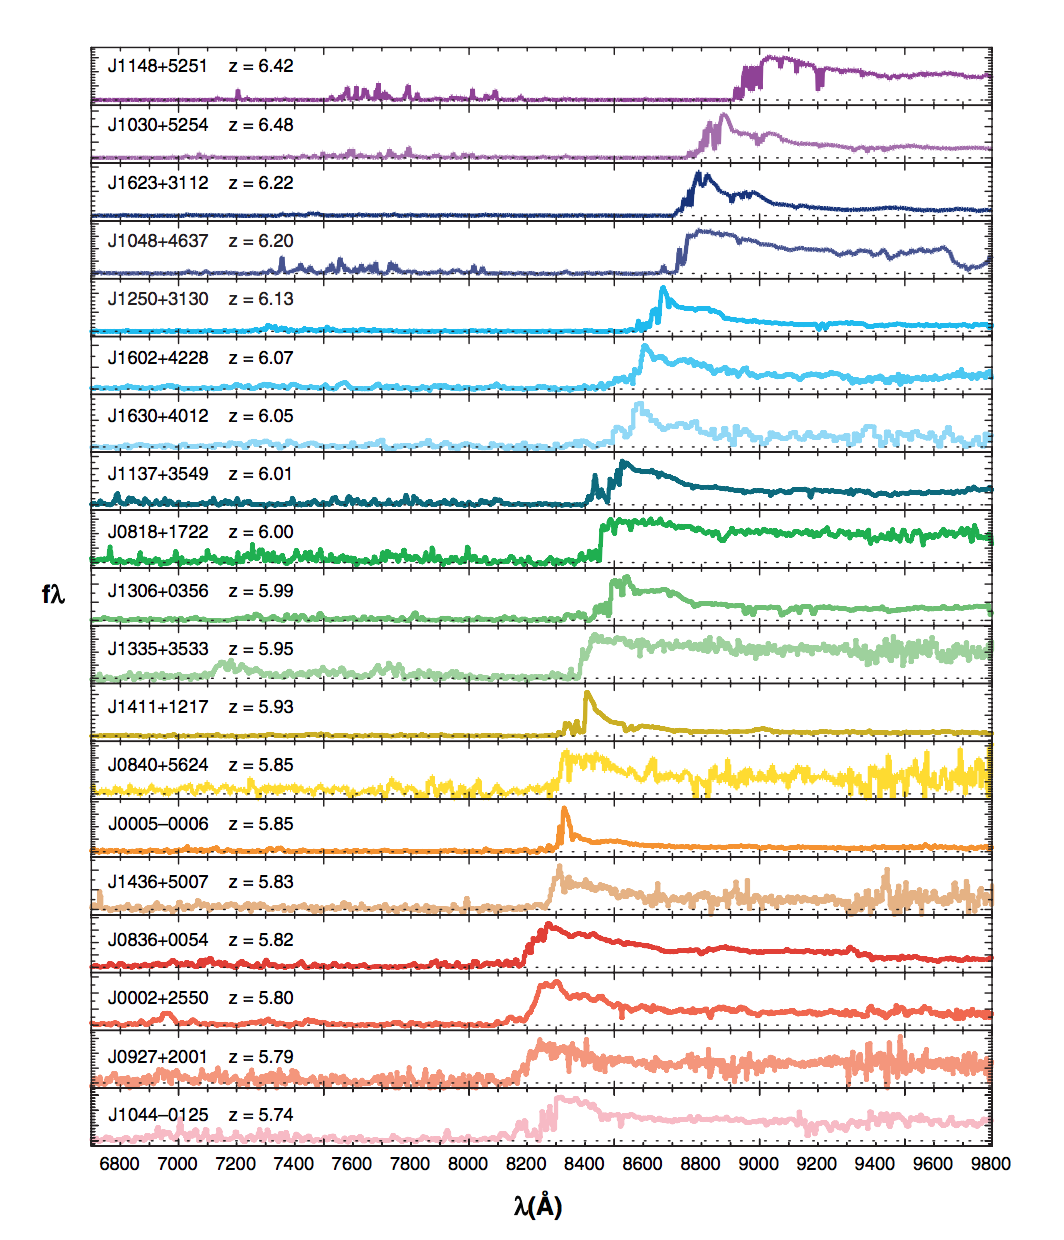
\includegraphics[width=0.8\textwidth]{chapters/eor_intro/figures/FanSpectra.png}
 \caption[The Ly$\alpha$ spectra of 19 high-redshift quasars.]{The Ly$\alpha$ spectra of 19 high-redshift quasars, as reported by \cite{Fan.06.2}. The effective optical depth towards each quasar increases with redshift, suggesting an evolution in the neutral fraction of the IGM. This figure was taken from \cite{Fan.06.review}.}
 \label{fig:eor_intro_qso}
 \end{figure}

Spectroscopic observations of high-redshift sources are relatively difficult to perform, and require large amounts of integration time. However, the distinctive Ly$\alpha$ limit in the spectra shown in Figure~\ref{fig:eor_intro_qso} is a distinctive property of high-redshift quasars. As an alternative, astronomers have developed a photometric method that is cheaper and easier to perform, called the ``Ly$\alpha$ dropout" technique. In this scheme, a survey will use an appropriate set of filters to probe a given redshift (imagine rectangles overlaid on the spectra in Figure~\ref{fig:eor_intro_qso}). If an excess is seen towards one galaxy in one filter, and very little signal is seen in the next-bluest filter, that galaxy may be considered a candidate high-$z$ quasar. With some modelling, the luminosity function of  Ly$\alpha$ dropout galaxies can be used to measure the mass distribution of galaxies as a function of redshift \citep[e.g.][]{Bouwens.15, Bouwens.16}. Using these luminosity functions and comparing to star formation rate models and measurements, \cite{Roberston.15} argue that current measurements are consistent with quasars playing a relatively minor role in reionization, with the bulk of ionizing photons arising form ``normal" galaxies rather than black hole accretion discs. However, this claim is moderately dependent upon uncertain model parameters, such as the escape fraction of ionizing photons from their local halo \citep{Robertson.13} and the star formation history at high redshifts. The latter is beginning to be answered as more high-redshift gamma-ray bursts are detected and characterized \citep{Wang.09, Robertson.12, Wang.15}\footnote{In work unrelated to the bulk of this thesis, I presented observations of gamma-ray burst hosts suggesting that gamma-ray bursts were unbiased tracers of star formation rate -- a crucial component for using gamma-ray bursts to inform our understanding of the EoR.}.

At the time of writing, photometric and spectroscopic observations of high-$z$ quasars suggest that the IGM had a neutral fraction $>10^{-4}$ at $z\sim 6$, indicating that the EoR ended around 1 Gyr after the Big Bang \citep{Barnett.17}. \cite{Fan.06.2} report a direction dependence on their measurements, suggesting that reionization was patchy, rather than homogeneous.

\subsection{Observations of the CMB}
% CMB tau, kSZ
CMB photons will Thomson-scatter off-of free electrons in their path, suppressing the amplitude of the observed primordial anisotropies by a factor of $e^{-\tau_{\rm re}}$. This optical depth is an integrated quantity, but the largest contribution to the integral will come from the large injection of free electrons into the IGM during the EoR.
% ME NO LIKEY
The effect is degenerate with the overall scaling of the total intensity power of the CMB, but if the free electron is within a quadrupolar anisotropy, it will also induce linear polarization in the CMB \citep{Zaldarriaga.97.pol}, boosting polarized power at specific spatial scales (the CMB is most-usefully described in harmonic $\ell$-space). \cite{Zaldarriaga.97.pol} show that the excess in polarized power should occur at $\ell\sim2\sqrt{\tau_{\rm re}}$. Polarized measurements of the CMB are able to leverage this effect to break the degeneracy between the optical depth and the overall scaling to obtain an estimate of $\tau_{re}$. If there were no anisotropies and no EoR, $\tau_{re}$ would not arise; its detection (the first of which is shown in Figure~XXX) confirms a scenario consistent with the EoR. The integral nature of $\tau_{re}$ ...

\section{Direct measurements of {\sc hi}}
\label{sec:eor_intro_hi}


% 21cm mechanism
% WF coupling
% UNPOLARIZED
% why is it interesting (near term) - Liu Tau constraints, Kittiswitt maps (topology of EoR = cool), Kern emulators -- sensitivity to astrophysics & cosmology

\subsection{Foreground Challenges}

% foreground sychtrotron and thermal noise

\subsection{Global spectrum}
% spectrum cartoon

%The 21 cm signal from the Epoch of Reionization (EoR) contains a wealth of information about the Universe at these early times, and can provide key insight inaccessible to other observational techniques \citep{Loeb.12}. 

In particular, the sky-averaged 21 cm signal, the so-called global signal, directly
contains key information about the thermal history of the intergalactic medium
(IGM) as a function of redshift \citep{Pritchard.10}. Historically,
observational efforts to detect the global signal have been ``single dish''
experiments, where a single receiving element is characterized to high
precision, and then operated in an effort to detect the EoR signal as a function
of frequency (and thus redshift). 

\subsubsection{Limits on the EoR} % change this title...

Experiments such as the Experiment to Detect
the Global EoR Step (EDGES, \citealt{Bowman.10}), Sonda Cosmol\'{o}gica
de las Islas para la Detecc\'{i}on de Hidr\'{o}geno Neutro (SCI-HI,
\citealt{Voytek.14}), and the Cosmic Twilight Polarimeter (CPT,
\citealt{Nhan.16}), have been proposed or constructed seeking to measure
the global signal from the Dark Ages or the EoR, through a deep understanding of
the properties of the instruments. In all cases, the instruments consist of a
single-element, and much of the observational effort contributes toward a
thorough understanding of systematic uncertainties of the instrument. 

%The signal from the Dark Ages and EoR is thought to be 4--5 orders of magnitude fainter than nearby bright foregrounds, such as galactic synchrotron radiation \citep{McQuinn.07}. As such, an exquisite understanding of the correlated noise in these instruments is of the utmost importance. Largely, these experiments have not yet detected a feature in frequency-space that can clearly be interpreted as a detection of either the Dark Ages or EoR global signal. To date, EDGES has provided a lower-limit on the duration of reionization of $\Delta z \geq 0.06$ \citep{Bowman.10}.

\subsection{Anisotropic signal}

\subsubsection{Current Limits}
% galaxies => z_end
% CMB => z_middle
% global limits => dz
% 

\section{Future probes}
\label{sec:eor_intro_future}
% 
% HI, CO, C+ intensity mapping, extreme deep fields from JWST [HIGH REDSHIFT SPECTROSCOPY? e.g. Salvaterra+ 2011]
% 


%
% what is the EoR -- history (global signal history)
% why is it interesting (near term) - Liu Tau constraints, Kittiswitt maps, Kern emulators -- sensitivity to astrophysics & cosmology
% "why do we think reionization ended at z=6?"
% --> hold cosmo params fixed, then we can constrain astro ones. If you want to constrain cosmology, we have some, weak, sensitivity (we have a complicated proxy for the density field)

% current (CMB tau, high-z galaxies (CANDELS; lyman alpha dropouts; quasars), Gunn Peterson, AHEM AHEM kSZ), EoR power spectrum, and future (HI, CO, C+ intensity mapping, extreme deep fields from JWST [HIGH REDSHIFT SPECTROSCOPY? e.g. Salvaterra+ 2011]) probes
% --> check out Mesinger paper trail and Robertson+'15
% current state of the art -- power spectra -- (limits from PAPER, LOFAR, MWA).


% why are we still looking => foregrounds -> relative signal scales -> more next chapter
% in the following chapters I will speak about...
%


% spectrum
% global signal - EDGES




% in the following chapters I will speak about...


\section{This thesis}
\label{sec:eor_intro_this_thesis}
Everything in this work -- algorithmic development, mathematical theory, observations -- was carried-out in order to facilitate the detection of the EoR. While these efforts took many forms, they shared that singular motivation of moving the field forward towards a detection of {\sc hi} at cosmological distances. 

This thesis is divided into three parts. Part {\sc i} is devoted to introducing concepts used throughout this work and building a mathematical formalism around those concepts. 
Chapter~\ref{chapter:astro_rad} reviews astrophysical mechanisms for producing polarized and unpolarized radiation at low radio frequencies. 
Chapter~\ref{chapter:interferometry} builds a formalism around measuring low frequency radio waves with interferometers (and the challenges associated with accurately measuring polarized radiation), and Chapter~\ref{chapter:instruments} introduces the instruments used throughout this work.

In Part {\sc ii} I present the bulk of my efforts: building an understanding of the imprint of the polarized sky, and the instrument itself, in the Fourier space used to set limits on the EoR power spectrum. 
Chapter~\ref{chapter:eor_window_theory} reviews the current theory and major results of mapping low frequency interferometric measurements into Fourier space. 
Chapter~\ref{chapter:data_prep_and_proc} details several required quality assurance and compression steps that must be taken to clean and interact with the data. Building from clean data, Chapter~\ref{chapter:polcal} presents new algorithms developed to calibrate the measurements.
Chapter~\ref{chapter:ionosphere} discusses the impact of Earth's ionosphere on our measurements.
In Chapters~\ref{chapter:eor_window_paper32img}, \ref{chapter:eor_window_HERA} and \ref{chapter:eor_window_psa128} I present successively-deeper integrations on polarized foregrounds in successively-narrower regions of Fourier space.

Part {\sc iii} explores other uses of EoR measurements, beyond detection of the power spectrum. In Chapter~\ref{chapter:TAV}, I discuss the potential of using long time-averages of interferometric measurements to measure some component of the monopole moment of the sky. In Chapter~\ref{chapter:ksz_21cm}, I present a new formalism for cross-correlating 21\,cm emission and CMB anisotropies in Fourier space. Chapter~\ref{chapter:hera_ml} describes my initial investigations into utilizing deep learning techniques for recovering cosmological parameters from simulated EoR measurements. I conclude in Chapter~\ref{chapter:conc}.
